% !TeX root = ../../main.tex
\section{Architecture}\label{section:architecture}

\begin{figure}[H]
  \centering
  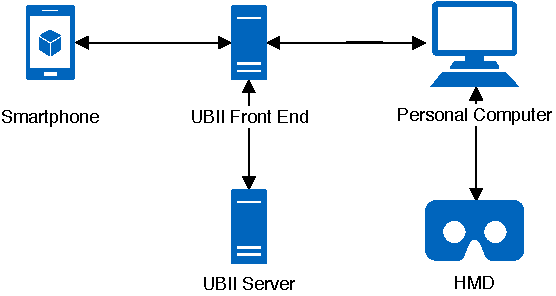
\includegraphics[width=10cm]{figures/implementation/architecture.pdf}
  \caption[The architecture of the system.]{The architecture of the system. An arrow means that the connected applications communicate over the network. The relevant software running on the devices are listed in brackets.}\label{fig:architecture}
\end{figure}

The experiments presented in the next Chapter are implemented as part of the \ac{UBII} front end. The same applies to the smart device client, as illustrated in Figure~\ref{fig:architecture}. Both applications run in a web browser on the device and communicate with the \ac{UBII} server\footnote{Figure~\ref{fig:architecture} illustrates no direct connection between the smartphone/\ac{PC} and the \ac{UBII} server for the sake of simplicity. However when running the software, one is actually established, since the \ac{UBII} front end runs on the client.}. In most scenarios, the connections of the smartphone are wireless ones over \ac{WLAN}. A \ac{PC} running the \ac{HMD} driver software and a web browser with the experiments open is used as a bridge between the \ac{HMD} and the \ac{UBII} front end. This setup may vary depending on the \ac{VR} headset. The Google Cardboard, for example, does not require any \ac{PC} in between.